\section{Our Approach}
\subsection{Data Description}
Our starting data set is a collection of 476 million tweets from June 2009 to December 2009. This data set was collected by Stanford University through their partnership with Twitter, and then later shared with other research teams. The data contains 17 million unique users. 

We begin our data analysis by performing several pre-processing steps to aid in our analysis . We first limit our dataset to English tweets from July and August of 2009, which totals 178 million tweets.  From these, we build a list of tweets containing at least one hashtag, which totals around 16 million tweets.  Next we remove all non-alphanumeric characters (e.g. commas, periods, etc.) to allow us to simply focus on the \emph{terms} (i.e. words, numbers) and hashtags being used in each tweet.  The number of unique hashtags over this time period is 872,402.  

The last step of  pre-processing was to remove several hashtags that are either auto-generated by external systems, or are \emph{micro-meme} hashtags, which are those used in no discernible pattern. An example of an auto-generated hashtag is $\#$fb which is appended by a particular Facebook application that shares posts on Facebook with Twitter. An example of a micro-meme hashtag would be $\#$followfriday, which is a weekly used hashtag by users to recommend other users of interest. 

From this pre-processed data, we are able generate a list of the most frequently used hashtags, along with the co-occurring frequencies of all hashtags and terms with each other. 

To simplify calculations during clustering, we limit ourselves to a subset of the top hashtags, along with all the hashtags they co-occur with. This is described in further detail in the Clustering Hashtags section. For our classification step, we limit our focus to a subset of tweets.


\subsection{Clustering Hashtags}
\subsubsection{Difficulties of Clustering}
Clustering is inherently a hard task, and clustering hashtags is no exception to this rule. There are a number of variables that make clustering hashtags very difficult. The first major difficulty is the fact that they are not required to be defined words. For example, the hashtag $\#$p2 is a popular marker if a tweet contains politically progressive thoughts. In most cases, hashtags are a concatenation of words such as $\#$iamthemob. There exist measures such as the Wu-Palmer distance and path distance similarity that are distances that are based on the synonyms of the words being examined. Unfortunately, this feature eliminates the possibility of using this measure as central component in a clustering algorithm, such as K-means. Our algorithm will still use this concept, but only in a very limited scope.

The fact that hashtags are usually concatenations also makes it difficult to apply another popular metric to compare words, known as Levenshtein distance (i.e. edit distance). As an example, this distance would say that the hashtags $\#$iamblessed and $\#$iamthemob are close to one another, when in reality, they are very different. We actually implemented a method centered on this distance, and the poor results backed this observation.

Further, the set of hashtags is constantly increasing in size, with new, ``trendy'' hashtags appear everyday. This fact forces us to create an algorithm that captures the essence of most hashtags used, while remain tractable. To account for this, we decided to focus our attention on the 2,000 most used hashtags, and clustered only over this set. This decision was a directly consequent of the final clustering algorithm, and will result in the clustering of more than 2,000 hashtags.

\subsubsection{Co-Occurrence Relation}
The paper written by J. Poschko developed the idea that two hashtags are similar if they co-occur in a tweet \cite{Poschko2011}. Intuitively, this concept makes sense. Two hashtags are inherently similar if they are contained in tweets that discuss the same topic, and this fact could not be any stronger than if they appear in the same exact tweet. To back this intuition, the paper calculates the Wu-Palmer distance between hashtags that co-occur, and shows that this value is higher than the distance between two randomly chosen words. It was mentioned previously that the Wu-Palmer distance is a poor distance for hashtags as a whole, since there would be many unknown distances between hashtags that are not words. However, it does provide a good measure if you only consider the set of hashtags that is made up of well-defined words. From this fact, we make the assumption that if the Wu-Palmer distance is high for reoccurring hashtags that are real words, then the set of all reoccurring hashtags can be used as baseline for a similarity measure.

After creating the co-occurring lists for the 2,000 most used hashtags, we used the natural language toolkit (NLTK) in python to find the Wu-Palmer distance for each hashtag in each list. We then took the average over all of the lists. The final value is found in Table 1, along with the baselines found by Poschko.
\begin{table}[ht]
\caption{}
\centering
\begin{tabular}{c c}
\hline\hline
& Average $S_{WP}$ \\ [0.5ex] % inserts table %heading
\hline
Co-Occurrences & .40 \\
Baseline (Random Words) & .16 \\[1ex]
\hline
\end{tabular}
\label{table:nonlin}
\end{table}
This table verifies that the claim by Poschko applies to our data set. Clearly, the hashtags found in co-occurrence list are much more similar than random words.
    
\subsubsection{Minimizing the Level of Noise}
However, even though this applies to the list as a whole, it does not mean that there is not still a considerable about of noise present. For example, $\#$photography is a popular hashtag one uses to denote a recently posted picture, and another hashtag is sometimes used to describe the place the picture is taken, such as $\#$iran. However, as this example illustrates, the fact that these hashtags co-occur does not mean that these two hashtags are similar by our definition of similarity. To help minimize the effect this has on later stages, let $n_{ij}$ be the total number of co-occurrences hashtag i has with hashtags j. Hashtags A and B are kept on the co-occurring list if and only if
\begin{eqnarray}
min (\frac{n_{AB}}{ \sum n_{Aj}}, \frac{n_{BA}} {\sum n_{Bj}}) > .05, \nonumber
\end{eqnarray}
otherwise it is removed from the list.

Even after this step, it is still possible that many noisy relations exist; therefore we do another level of filtering, by comparing the contents of the respective co-occurring lists. Let m be the total number of hashtags that occur in both hashtag A and hashtag B co-occurrence lists. Further, let $m_A$ be the total number of occurrences of these hashtags in list A, and $m_B$ be the total number of occurrences in list B. Then the relationship between hashtag A and hashtag B is maintained if an only if
\begin{eqnarray}
min (\frac{{m_A} }{\sum n_{Aj}}, \frac{m_B }{ \sum n_{Bj}} ) > .2. \nonumber
\end{eqnarray}
Note that by the first level of filtering, this minimum is at least .05. Comparing each list takes a considerable amount of time to run, and this bottleneck forced us to constrain our focus to only 2,000 hashtags. However, it is easily parallelizable, and when program efficiently, would allow a much greater number of hashtags to be considered.

\subsubsection{Defining the Similarity Measure}
Using the Wu-Palmer distance and filtering methods described, we are confident the lists of co-occurring hashtags that remain imply some level of similarity between hashtags in these lists. As a result, we define the following similarity measure between hashtags A and hashtags B:
\begin{eqnarray}
S(A,B) = ( \frac{n_{AB}}{\sum n_{Aj}} + \frac{n_{BA} } {\sum n_{Bj}}) /2 . \nonumber
\end{eqnarray}
This function fits the axioms of a similarity measure. S(A,B) = S(B,A), and S(A,B) $\geq$ 0, and based on filtering process it will actually be greater than .05. It should be noted that several similarity measures were tested, such as multiplying the two ratios together, but this proved to be the best measure.

\begin{figure}[tbh]
\centering
\subfigure[]{
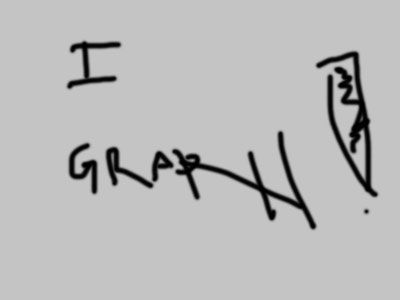
\includegraphics[scale=0.20]{./wordGraphs/slide1.jpg}
}
\subfigure[]{
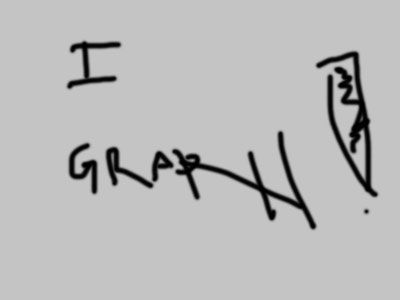
\includegraphics[scale=0.20]{./wordGraphs/slide2.jpg}
}
\subfigure[]{
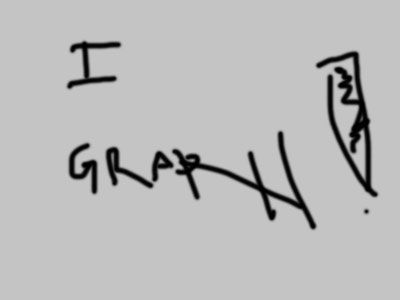
\includegraphics[scale=0.20]{./wordGraphs/slide3.jpg}
}
\subfigure[]{
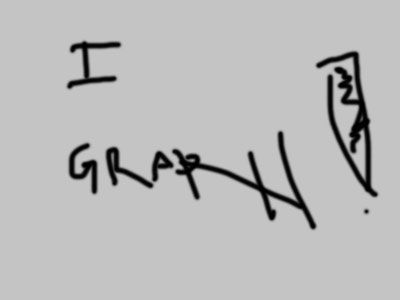
\includegraphics[scale=0.20]{./wordGraphs/slide4.jpg}
}
\subfigure[]{
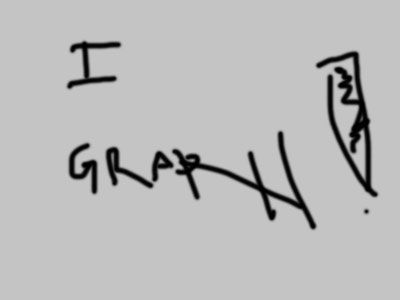
\includegraphics[scale=0.20]{./wordGraphs/slide5.jpg}
}
\subfigure[]{
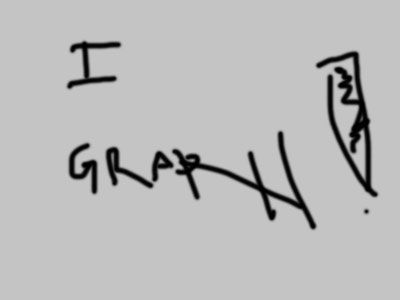
\includegraphics[scale=0.20]{./wordGraphs/slide6.jpg}
}
\caption{Subfigure (a) represents the original undirected graph proposed by the co-occurring lists. Subfigures (b) and (c) consists of only the neighbors of apple and iphone respectively (the graph remains undirected). Subfigures (d) and (e) convert the undirected graphs into an directed graph by weighing the edges. The filter process examines these directed graphs, and after passing the final undirected graph with the similarity measure is created (f).}
\label{fig:words}
\end{figure}

\subsubsection{Spectral Clustering and METIS}
With our well defined similarity measure, and thus similarity matrix, spectral clustering was the ideal candidate to perform clustering over our list of hashtags. For comparison purposes, we performed spectral clustering and normalized spectral clustering. We also examined a graph program named METIS that claimed to perform 10$\%$ to 50$\%$ better than spectral algorithms \cite{Karypis1999}. This algorithm is based on multilevel recursive-bisection and multilevel k-way partitioning schemes. Instead of using an Laplacian matrix like the spectral methods, METIS takes in the similarity matrix, and uses the similarity measures to define a weighted graph.

\subsection{Classification}
\setcounter{secnumdepth}{4}

In the classification step, we will attempt to classify various tweets into classes defined by the hashtag clusters. Intuitively, the idea is that given the text of a tweet, the classification algorithms will be able to ``suggest'' what hashtags it should contain. Since we have actually clustered the hashtags, we will not be suggesting what hashtags the tweet will contain, but will suggest which cluster the hashtag is most likely to fall into.  

\subsubsection{Description of feature vectors and classes}
For classification, we have a corpus of text tweets that we will map to clusters of hashtags. We can consider each tweet a document and use standard document classification techniques in this step. We create a dictionary of all unique words (removing common stop words and all hashtags) that occur in all the tweets. Let us assume that there are {\it d} words in the dictionary.  
The feature vector is a {\it d}-dimensional integer-valued vector where the {\it $i^{th}$} entry in the vector represents the frequency of the {\it i$^{th}$} word in the tweet.

The classes that each feature vector is classified into is represented by the hashtag clusters. A tweet belongs to a class if a hashtag appearing in the tweet is part of a certain cluster. When generating the training data, if a tweet has multiple hashtags, we consider that tweet to be a part of multiple classes so we add the same training point multiple times with different classes as the target. We do this since the text of a tweet is related to all the hashtags in the tweet.  

Due to the size of our training sets, each feature vector was an extremely-sparse high-dimensional vector. Due to the number of training samples and the high dimensionality of the vector, attempting to classify over the complete data was intractable on any machines that we had access to. To get around this problem, we used two solutions.


\subsubsection{Classification using Dimensionality Reduction}

We used a software package for Python named {\it scikit-learn} to reduce the dimensions in our data. For our dataset containing 100,000 tweets, we had approximately 46,000 dimensions. We reduced this to 100 dimensions using PCA. Once we had reduced the number of dimensions, it was possible to apply some standard classification algorithms to the data. We applied the following algorithms to the reduced-dimension data.

\paragraph{Naive Bayes.}
Applying the Naive Bayes algorithm, we were getting very poor performance. This is because PCA creates real-valued feature vectors whose values don't always mean much. Hence we binarized the data using a simple strategy: all positive values in the feature vector took the value 1, and all negative values took the value 0. Using this new data we were able to get reasonable performance using the Naive Bayes classification algorithm.

\paragraph{Linear Discriminant Analysis.}
When using LDA, we were able to get acceptable performance using just the reduced-dimension data. We didn't need to create a binary representation of the data.

\subsubsection{Classification using SVM algorithm optimized for sparse vectors}
Another method we used to circumvent the high dimensionality of the feature vectors was using an algorithm that was designed to use the sparse representation of a vector. By representing the feature vectors as a sparse vector, the problem becomes tractable and we don't need to do any dimensionality reduction. We used a Radial Basis Function as the kernel for the SVM. Since SVM is an inherently a binary classifier, we use a one-versus-all strategy to make it a multi-class classifier. This was also implemented using the software package {\it scikit-learn}.

\subsubsection{Majority Vote classification}
As a baseline measure, we also did classification by majority vote. This method simply involved looking at all the training data, and predicting each test point that class which occured most in the training data.